\section{Introduction}\label{sec:intro}
In this project, a Quanser helicopter model was analysed and controlled using fundamental considerations from linear system theory. Important concepts from control theory and estimation theory were applied to achieve robust and responsive control of the helicopter. 

Among the controllers studied were both a classical feedback controller with proportional and derivative effect, as well as a linear quadratic regulator. The latter was implemented with both reference feed forward as well as integral effect, but not at the same time. 

In addition to implementing and tuning the controllers, the system was analysed for its observability and controllability when placed under different constraints. For instance, in part IV, the observability was analysed for different number of output variables. Linear observers were also used to test the controllers with estimated instead of measured state.

\section{Problem Description}\label{sec:prob_descr}
The problems revolves around a physical model of a helicopter arm which is fasten to the ground and has three degrees of freedom. Elevation ($e$), pitch ($p$) and travel ($\lambda$). 
The helicopter was controlled through a joystick and interfaced to the helicopter with \MATLAB and Quanser's \QuaRC Real-Time Control Software. The following tasks are described in the report:

\begin{itemize}
    \item Mathematical modelling of the system.
    \item Control of the system with mono- and multivariable controllers
    \item Synthesis of a linear quadratic regulator (LQR) for the system
    \item State estimation for states that are not directly measured 
\end{itemize}

The helicopter can be modeled as three point masses: two masses represent the motors of the propellers and the third is the counterweight on the opposite side. Refer to \cref{fig:heli} and \cref{fig:heli_dimensions} for depiction of setup. The cylindres in \cref{fig:heli} are the joints where the axis of the cylindres are equal to the axis of rotation of the joint. The following definitions are made: \textit{p} is the pitch angle of the helicopter head, \textit{e} is its elevation angle and \textit{$\lambda$} is the travel angle of the helicopter. Fig. \ref{fig:heli} shows all angles at zero and with positive orientation as indicated. For the sake of this report, it is assumed that there is a linear relationship between the forces the propellers generate and the voltage that is applied to them:

\begin{subequations}\label{eq:P1_forces_propellers}
    \begin{align}
        F_f&=K_f V_f     \label{eq:P1_forces_propellers_f} \\
        F_b&=K_f V_b     \label{eq:P1_forces_propellers_b}
    \end{align}
\end{subequations}
The proportionality constant, $K_f$, is called the \textit{motor constant}. 

Additionally, it is assumed that the weights of the motors and the counterweight are given as:
\begin{subequations}\label{eq:P1_weights}
    \begin{align}
        F_{g,f}=F_{g,b}&= m_pg   \label{eq:P1_weight_m_p} \\
                F_{g,c}&=m_cg    \label{eq:P1_weight_m_c}
    \end{align}
\end{subequations}

The propellers are placed symmetrically in relation to the pitch axis and the forces always attack perpendicular to the plane made by the pitch and elevation axis. The weight of the point masses are called $F_{g,f}, F_{g,b}$ and $F_{g,c}$ and attack parallel to gravity.

For the sake of this report, it is assumed that the weight of the two propeller motors are equal and given by $m_p$. The counterweight mass is indicated by $m_c$. The distance along the elevation axis between the travel axis and pitch axis is indicated by $l_h$. The length from the travel axis to the counterweight is indicated by $l_c$. 

Further simplifications to the helicopter model have been made, such as neglect of the (quite prominent) \text{ground effect}.\cite{CheesemanGregory} 

\begin{figure}[bp]
	\centering
	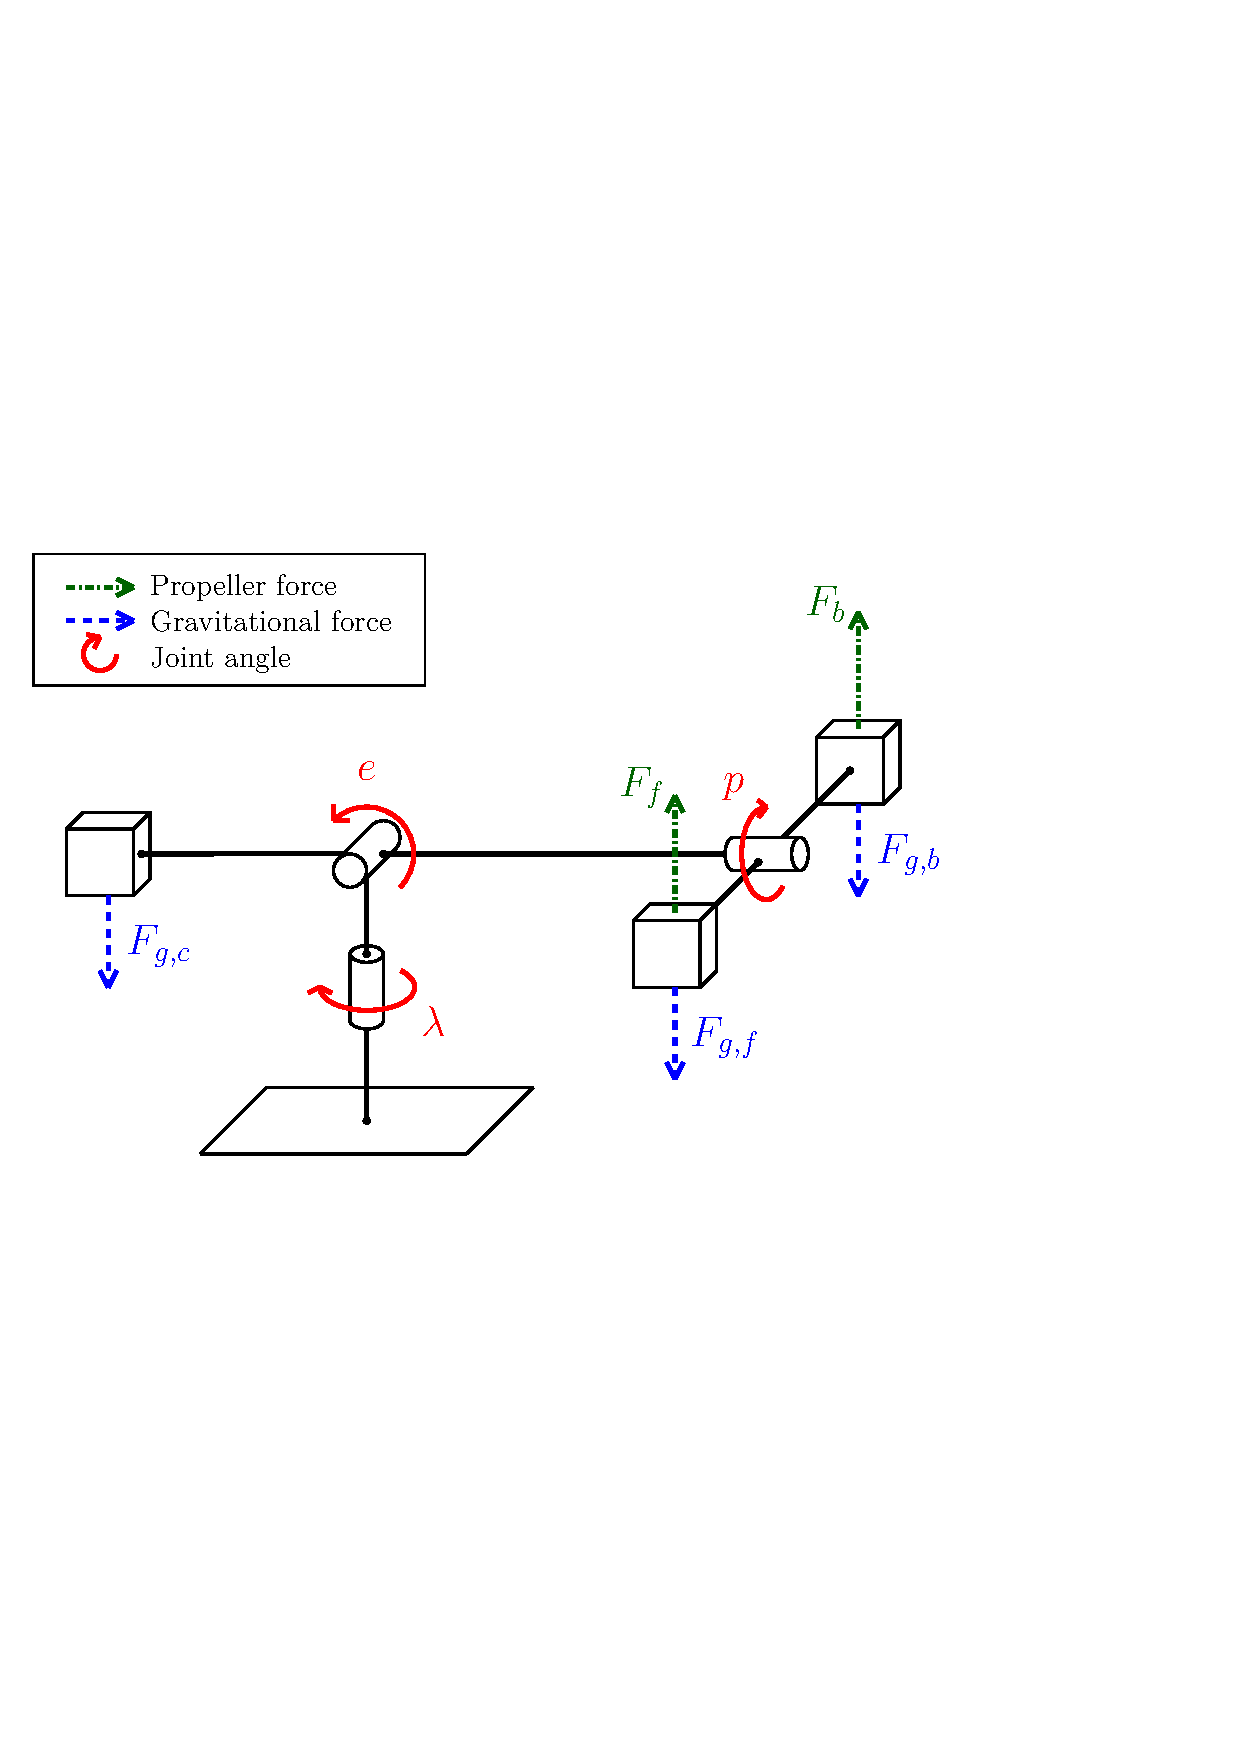
\includegraphics[width=0.80\textwidth]{figures/forces.pdf}
	\caption{Depiction of model of system. Force directions and positive angles are defined as indicated.}
\label{fig:heli}
\end{figure}

\begin{figure}[bp]
	\centering
	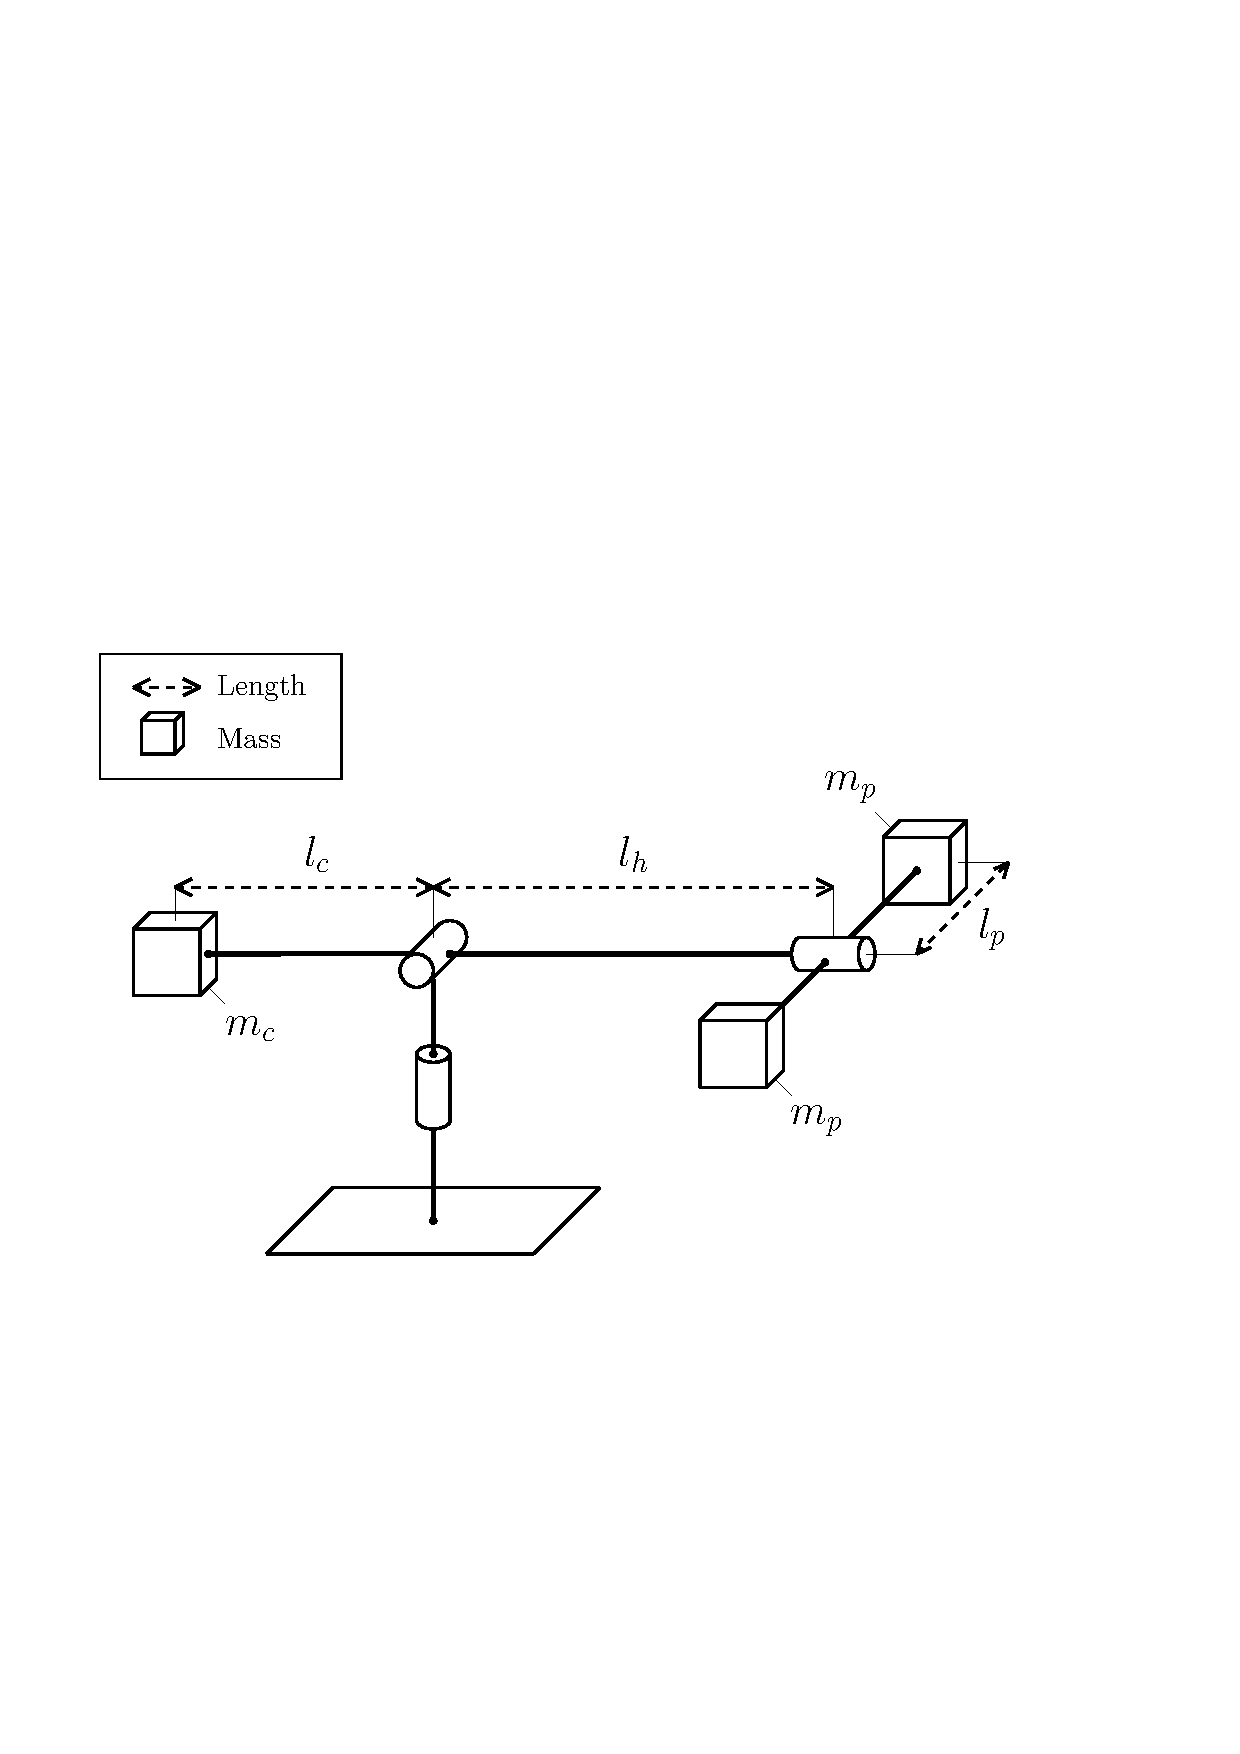
\includegraphics[width=0.80\textwidth]{figures/helicopter.pdf}
	\caption{Depiction of all lengths and masses of the system.}
\label{fig:heli_dimensions}
\end{figure}

The report is divided into four parts. The first part will make mathematical descriptions of the described system. Part II will describe the implementation of monovariable control through the use of PD and P controllers. Part III will describe the implementation of an LQR controller and lastly, Part IV will describe the implementation of a state estimation model into the LQR controller.